\section{The Spatial Language}
\label{language}

Spatial is a domain specific language for the design of accelerators implemented on reconfigurable spatial architectures, including FPGAs and CGRAs.
The aim of the language is to simplify the accelerator design process,
allowing domain experts to quickly develop, test, optimize, and deploy hardware accelerators, either by
directly implementing high-level hardware designs or by targeting Spatial from another, higher level language.

%When used to target FPGAs, the output of Spatial is a target-specific, synthesizable Chisel project, meaning users can go directly from a Spatial program to a design running on their target device.
%Spatial is currently implemented as an embedded language in Scala.
%Spatial employs a mix of imperative and functional paradigms to improve the amount of information available to the compiler.
In this section, we describe the abstractions Spatial includes to balance productivity and performance-oriented detail.
While space does not permit a full specification of the language, Table~\ref{t:syntaxTable} provides an overview of the core subset of Spatial's syntax.
%including control structures, optional user scheduling directives, memory templates for various levels of the memory hierarchy, and design space parameters.


%A higher level language targeted towards hardware accelerator design must strike the right balance
%between high-level abstractions for improving programmer productivity and target-specific constructs for controlling hardware performance.

%In this section, we discuss several of the key challenges in defining hardware accelerator designs and describe abstractions the Spatial language includes to place the burden of this complexity on the compiler rather than the application programmer.

\newcommand{\desyntax}{\vspace{-10pt}}
\newcommand{\syntaxtitle}[1]{
\multicolumn{1}{l}{\bf{#1}} \vspace{-6pt} \\
\hspace{-4pt}\rule{0.48\columnwidth}{.4pt} \\
}

\begin{table*}
\centering

%%%%%%%%% ----- Counter ------- %%%%%
\newsavebox{\counter}
\begin{lrbox}{\counter}
\begin{lstlisting}[language=SpatialTable]
min* until max by stride* par p* : Counter
\end{lstlisting}
\end{lrbox}

%%%%%%%%% ----- FSM ------- %%%%%
\newsavebox{\fsmSignature}
\begin{lrbox}{\fsmSignature}
\begin{lstlisting}[language=SpatialTable]
FSM(init){while}{f}{next}: Void
\end{lstlisting}
\end{lrbox}

%%%%%%%%% ----- Foreach ------- %%%%%
\newsavebox{\foreachSignature}
\begin{lrbox}{\foreachSignature}
\begin{lstlisting}[language=SpatialTable]
Foreach(counter+){f}: Void
\end{lstlisting}
\end{lrbox}

%%%%%%%%% ----- Reduce ------- %%%%%
\newsavebox{\reduceSignature}
\begin{lrbox}{\reduceSignature}
\begin{lstlisting}[language=SpatialTable]
Reduce(accum)(counter+){f}{r}: Reg[T]
\end{lstlisting}
\end{lrbox}

%%%%%%%%% ----- MemReduce ------- %%%%%
\newsavebox{\memreduceSignature}
\begin{lrbox}{\memreduceSignature}
\begin{lstlisting}[language=SpatialTable]
MemReduce(accum)(counter+){f}{r}: SRAM$^M$[T]
\end{lstlisting}
\end{lrbox}

%%%%%%%%% ----- Stream ------- %%%%%
\newsavebox{\streamStar}
\begin{lrbox}{\streamStar}
\begin{lstlisting}[language=SpatialTable]
Stream(*){f}: Void
\end{lstlisting}
\end{lrbox}

%%%%%%%%% ----- Parallel ------- %%%%%
\newsavebox{\parallelSignature}
\begin{lrbox}{\parallelSignature}
\begin{lstlisting}[language=SpatialTable]
Parallel{f}: Void
\end{lstlisting}
\end{lrbox}

%%%%%%%%% ----- DummyPipe ------- %%%%%
\newsavebox{\pipeSignature}
\begin{lrbox}{\pipeSignature}
\begin{lstlisting}[language=SpatialTable]
DummyPipe{f}: Void
\end{lstlisting}
\end{lrbox}

%%%%%%%%% ----- IfThenElse ------- %%%%%
\newsavebox{\ifSignature}
\begin{lrbox}{\ifSignature}
\begin{lstlisting}[language=SpatialTable]
if (cond$_1$){f$_1$}
else if (cond$_i$){f$_i$} +
else {f$_N$}* : T
\end{lstlisting}
\end{lrbox}

%%%%%%%%% ----- Sequential Tag ------- %%%%%
\newsavebox{\sequentialTag}
\begin{lrbox}{\sequentialTag}
\begin{lstlisting}[language=SpatialTable]
Sequential.(Foreach|Reduce|MemReduce)
\end{lstlisting}
\end{lrbox}

%%%%%%%%% ----- Pipe Tag ------- %%%%%
\newsavebox{\pipeTag}
\begin{lrbox}{\pipeTag}
\begin{lstlisting}[language=SpatialTable]
Pipe(ii*).(Foreach|Reduce|MemReduce)
\end{lstlisting}
\end{lrbox}

%%%%%%%%% ----- Stream Tag ------- %%%%%
\newsavebox{\streamTag}
\begin{lrbox}{\streamTag}
\begin{lstlisting}[language=SpatialTable]
Stream.(Foreach|Reduce|MemReduce)
\end{lstlisting}
\end{lrbox}

%%%%%%%%% ----- Parallel Tag ------- %%%%%
\newsavebox{\parallelTag}
\begin{lrbox}{\parallelTag}
\begin{lstlisting}[language=SpatialTable]
Parallel.(Foreach|Reduce|MemReduce)
\end{lstlisting}
\end{lrbox}

%%%%%%%%% ----- FIFO ------- %%%%%
\newsavebox{\fifoSyntax}
\begin{lrbox}{\fifoSyntax}
\begin{lstlisting}[language=SpatialTable]
FIFO[T](depth)
\end{lstlisting}
\end{lrbox}

%%%%%%%%% ----- LIFO ------- %%%%%
\newsavebox{\filoSyntax}
\begin{lrbox}{\filoSyntax}
\begin{lstlisting}[language=SpatialTable]
LIFO[T](depth)
\end{lstlisting}
\end{lrbox}

%%%%%%%%% ----- LineBuffer ------- %%%%%
\newsavebox{\lineBufferSyntax}
\begin{lrbox}{\lineBufferSyntax}
\begin{lstlisting}[language=SpatialTable]
LineBuffer[T](r, c)
\end{lstlisting}
\end{lrbox}

%%%%%%%%% ----- LUT ------- %%%%%
\newsavebox{\lutSyntax}
\begin{lrbox}{\lutSyntax}
\begin{lstlisting}[language=SpatialTable]
LUT[T](dim+)(elements+)
\end{lstlisting}
\end{lrbox}

%%%%%%%%% ----- Reg ------- %%%%%
\newsavebox{\regSyntax}
\begin{lrbox}{\regSyntax}
\begin{lstlisting}[language=SpatialTable]
Reg[T](reset*)
\end{lstlisting}
\end{lrbox}

%%%%%%%%% ----- RegFile ------- %%%%%
\newsavebox{\regfileSyntax}
\begin{lrbox}{\regfileSyntax}
\begin{lstlisting}[language=SpatialTable]
RegFile[T](dim+)
\end{lstlisting}
\end{lrbox}

%%%%%%%%% ----- SRAM ------- %%%%%
\newsavebox{\sramSyntax}
\begin{lrbox}{\sramSyntax}
\begin{lstlisting}[language=SpatialTable]
SRAM[T](dim+)
\end{lstlisting}
\end{lrbox}

%%%%%%%%% ----- ArgIn ------- %%%%%
\newsavebox{\argInSyntax}
\begin{lrbox}{\argInSyntax}
\begin{lstlisting}[language=SpatialTable]
ArgIn[T]
\end{lstlisting}
\end{lrbox}

%%%%%%%%% ----- ArgOut ------- %%%%%
\newsavebox{\argOutSyntax}
\begin{lrbox}{\argOutSyntax}
\begin{lstlisting}[language=SpatialTable]
ArgOut[T]
\end{lstlisting}
\end{lrbox}

%%%%%%%%% ----- HostIO ------- %%%%%
\newsavebox{\hostIOSyntax}
\begin{lrbox}{\hostIOSyntax}
\begin{lstlisting}[language=SpatialTable]
HostIO[T]
\end{lstlisting}
\end{lrbox}

%%%%%%%%% ----- DRAM ------- %%%%%
\newsavebox{\dramSyntax}
\begin{lrbox}{\dramSyntax}
\begin{lstlisting}[language=SpatialTable]
DRAM[T](dim+)
\end{lstlisting}
\end{lrbox}

%%%%%%%%% ----- StreamIn ------- %%%%%
\newsavebox{\streamInSyntax}
\begin{lrbox}{\streamInSyntax}
\begin{lstlisting}[language=SpatialTable]
StreamIn[T](bus)
\end{lstlisting}
\end{lrbox}

%%%%%%%%% ----- StreamOut ------- %%%%%
\newsavebox{\streamOutSyntax}
\begin{lrbox}{\streamOutSyntax}
\begin{lstlisting}[language=SpatialTable]
StreamOut[T](bus)
\end{lstlisting}
\end{lrbox}

%%%%%%%%% ----- Parameter ------- %%%%%
\newsavebox{\parameterSyntax}
\begin{lrbox}{\parameterSyntax}
\begin{lstlisting}[language=SpatialTable]
default (min,step*,max)
\end{lstlisting}
\end{lrbox}

%%%%%%%%% ----- Accel ------- %%%%%
\newsavebox{\accelSyntax}
\begin{lrbox}{\accelSyntax}
\begin{lstlisting}[language=SpatialTable]
Accel{body}
\end{lstlisting}
\end{lrbox}

%%%%%%%%% ----- Accel* ------- %%%%%
\newsavebox{\accelStarSyntax}
\begin{lrbox}{\accelStarSyntax}
\begin{lstlisting}[language=SpatialTable]
Accel(*){body}
\end{lstlisting}
\end{lrbox}


\fontsize{8}{10}
\selectfont
\hspace{-10pt}
\begin{tabular}{m{0.45\columnwidth} m{0.01\columnwidth} m{0.45\columnwidth}}
\begin{tabular}{l}

\syntaxtitle{(a) Control Structures}

\multirow{1}{*}{\usebox{\counter}} \\
\vspace{-7pt} \\
A counter over $[\argg{min},\argg{max})$.  \\
\vspace{-8pt} \\
{
\begin{tabular}{lll}
\argg{min}:  &\hspace{-10pt}$\mathbb{Z}$ & \hspace{-4pt}Start value, inclusive. Default is 0. \\
\argg{max}:  &\hspace{-10pt}$\mathbb{Z}$ & \hspace{-4pt}Counter maximum, non-inclusive. \\
\argg{step}: &\hspace{-10pt}$\mathbb{Z}$ & \hspace{-4pt}Counter stride. Default is 1. \\
\argg{p}:    &\hspace{-10pt}$\mathbb{Z}$ & \hspace{-4pt}Counter parallelization. Default is 1. \\
\end{tabular}
} \\ \desyntax\\

% \multirow{3}{*}{\usebox{\ifSignature}} \\ \\ \\
% \vspace{-7pt} \\
% Data-dependent execution of first valid condition. \\
% Doubles as a multiplexer if $T \in \mathbb{B}$. \\
% \vspace{-8pt} \\
% {
% \begin{tabular}{lll}
% \argg{cond$_i$}: &\hspace{-10pt} $\rightarrow$ \scalar{T} & \hspace{-4pt}Condition for associated body. \\
% \argg{f$_i$}: &\hspace{-10pt} $\rightarrow$ \scalar{T} & \hspace{-4pt}Arbitrary expression. \\
% \end{tabular}
% } \\ \desyntax\\

\multirow{1}{*}{\usebox{\fsmSignature}} \\
\vspace{-7pt} \\
An arbitrary finite state machine. \\
Internal state is a value of type $T \in \mathbb{B}$ \\
\vspace{-8pt} \\
{
\begin{tabular}{lll}
\argg{init}:   &\hspace{-10pt} \scalar{T} & \hspace{-4pt}The FSM's initial state.  \\
\argg{while}:  &\hspace{-10pt} \scalar{T} $\rightarrow$ \scalar{Bit}  & \hspace{-4pt}Continue function.  \\
\argg{f}:      &\hspace{-10pt} \scalar{T} $\rightarrow$ \scalar{Void} & \hspace{-4pt}Function executed each iteration.  \\
\argg{next}    &\hspace{-10pt} \scalar{T} $\rightarrow$ \scalar{T}    & \hspace{-4pt}State transition function. \\
\end{tabular}
} \\ \desyntax\\

\multirow{1}{*}{\usebox{\foreachSignature}} \\
\vspace{-7pt} \\
A parallelizable \emph{for} loop. \\
\vspace{-8pt} \\
{
\begin{tabular}{lll}
\argg{counter}: &\hspace{-10pt} \texttt{\textcolor{darkgreen}{Counter$_D$}} & \hspace{-4pt}Loop iteration domain.    \\
\argg{f}:       &\hspace{-10pt} $\mathbb{Z}_D \rightarrow $ \scalar{Void}   & \hspace{-4pt}Loop body. \\
\end{tabular}
} \\ \desyntax\\

\multirow{1}{*}{\usebox{\reduceSignature}} \\
\vspace{-7pt} \\
A reduction of scalars $T \in \mathbb{B}$, parallelized as a tree. \\
\vspace{-8pt} \\
{
\begin{tabular}{lll}
\argg{accum}:   &\hspace{-10pt} \memory{Reg}\texttt{[}\scalar{T}\texttt{]}       & \hspace{-4pt}Accumulation register.    \\
\argg{counter}: &\hspace{-10pt} \memory{Counter$_D$}                             & \hspace{-4pt}Loop iteration domain.    \\
\argg{f}:       &\hspace{-10pt} $\mathbb{Z}_D \rightarrow$ \scalar{T}            & \hspace{-4pt}Map function. \\
\argg{r}:       &\hspace{-10pt} (\scalar{T},\scalar{T}) $\rightarrow$ \scalar{T} & \hspace{-4pt}Combinination function. \\
\end{tabular}
} \\ \desyntax\\

\multirow{1}{*}{\usebox{\memreduceSignature}} \\
\vspace{-7pt} \\
Reduction over $M$-dimensional memories. \\
\vspace{-8pt} \\
{
\begin{tabular}{lll}
\argg{accum}:   &\hspace{-10pt} \memory{SRAM$^M$}\texttt{[}\scalar{T}\texttt{]} & \hspace{-4pt}Accumulation memory.    \\
\argg{counter}: &\hspace{-10pt} \texttt{\textcolor{darkgreen}{Counter$_D$}} & \hspace{-4pt}Loop iteration domain.    \\
\argg{f}:       &\hspace{-10pt} $\mathbb{Z}_D \rightarrow$ \memory{SRAM$^M$}\texttt{[}\scalar{T}\texttt{]}  & \hspace{-4pt}Map function. \\
\argg{r}:       &\hspace{-10pt} (\scalar{T},\scalar{T}) $\rightarrow$ \scalar{T}         & \hspace{-4pt}Combination function. \\
\end{tabular}
} \\ \desyntax\\

\multirow{1}{*}{\usebox{\streamStar}} \\
\vspace{-7pt} \\
A streaming loop which never terminates. \\
\vspace{-8pt} \\
{
\begin{tabular}{lll}
\argg{f}:   &\hspace{-10pt} $\rightarrow$ \scalar{Void} & \hspace{-4pt}Arbitrary expression. \\
\end{tabular}
} \\ \desyntax\\

\multirow{1}{*}{\usebox{\parallelSignature}} \\
\vspace{-7pt} \\
Overrides normal compiler scheduling. All conrollers \\
are instead scheduled in a \emph{fork-join} fashion. \\
\vspace{-8pt} \\
{
\begin{tabular}{lll}
\argg{f}:   &\hspace{-10pt} $\rightarrow$ \scalar{Void} & \hspace{-4pt}Arbitrary sequence of controllers. \\
\end{tabular}
} \\ \\

% \multirow{1}{*}{\usebox{\pipeSignature}} \\
% \vspace{-7pt} \\
% A ``loop'' with exactly one iteration. \\
% Inserted by the compiler, generally not written explicitly. \\
% \vspace{-8pt} \\
% {
% \begin{tabular}{lll}
% \argg{f}:   &\hspace{-10pt} $\rightarrow$ \scalar{Void} & \hspace{-4pt}Arbitrary expression. \\
% \end{tabular}
% } \\ \desyntax\\

\syntaxtitle{(b) Optional Scheduling Directives}

\multirow{1}{*}{\usebox{\sequentialTag}} \\
\vspace{-7pt} \\
Sets loop to run sequentially. \\
\desyntax\\

\multirow{1}{*}{\usebox{\pipeTag}} \\
\vspace{-7pt} \\
Sets loop to be pipelined. \\
{
\begin{tabular}{lll}
\argg{ii}:   &\hspace{-10pt} $\mathbb{Z}$ & \hspace{-4pt}Optional initiation interval . \\
\end{tabular}
}
\\ \desyntax\\

\multirow{1}{*}{\usebox{\streamTag}} \\
\vspace{-7pt} \\
Sets loop to be streaming. \\

\end{tabular} & &
\begin{tabular}{l}

\syntaxtitle{(c) On-Chip Memories}

\multirow{1}{*}{\usebox{\fifoSyntax}} \\
\vspace{-7pt} \\
FIFO with \argg{depth} elements of type \scalar{T}. \\
{
\begin{tabular}{lll}
\argg{depth}: &\hspace{-10pt} $\mathbb{Z}$ & \hspace{-4pt}Capacity of FIFO. \\
\end{tabular}
}
\\ \desyntax\\
%
% \multirow{1}{*}{\usebox{\filoSyntax}} \\
% A LIFO (stack) with a capacity of \argg{depth} elements of type \argg{T} \\
% \desyntax \\

% \multirow{1}{*}{\usebox{\lineBufferSyntax}} \\
% \vspace{-7pt} \\
% Buffer containing \argg{r} ``lines'' of \argg{c} elements. \\
% {
% \begin{tabular}{lll}
% \argg{r}: &\hspace{-10pt} $\mathbb{Z}$ & \hspace{-4pt}Number of lines. \\
% \argg{c}: &\hspace{-10pt} $\mathbb{Z}$ & \hspace{-4pt}Elements per line. \\
% \end{tabular}
% }
% \\ \desyntax\\
%
% \multirow{1}{*}{\usebox{\lutSyntax}} \\
% Read-only Lookup Table containing supplied \argg{elements} of type \argg{T} \\
% \vspace{-10pt}\\

\multirow{1}{*}{\usebox{\regSyntax}} \\
\vspace{-7pt} \\
Register holding a value of type \argg{T}. \\
{
\begin{tabular}{lll}
\argg{reset}: &\hspace{-10pt} \scalar{T} & \hspace{-4pt}Optional reset value. \\
\end{tabular}
}
\\ \desyntax \\

\multirow{1}{*}{\usebox{\regfileSyntax}} \\
\vspace{-7pt} \\
$D$-dimensional register file of elements of type \scalar{T}.\\
{
\begin{tabular}{lll}
\argg{dim}: &\hspace{-10pt} $\mathbb{Z}_D$ & \hspace{-4pt}Memory dimensions. \\
\end{tabular}
}
\\ \desyntax \\

\multirow{1}{*}{\usebox{\sramSyntax}} \\
\vspace{-7pt} \\
$D$-dimensional scratchpad of elements of type \scalar{T}. \\
{
\begin{tabular}{lll}
\argg{dim}: &\hspace{-10pt} $\mathbb{Z}_D$ & \hspace{-4pt}Memory dimensions. \\
\end{tabular}
}
\\ \\


\syntaxtitle{(d) Shared Host/Accelerator Memories}

\multirow{1}{*}{\usebox{\argInSyntax}} \\
\vspace{-7pt} \\
Accelerator register initialized by the host. \\
\desyntax\\

\multirow{1}{*}{\usebox{\argOutSyntax}} \\
\vspace{-7pt} \\
Accelerator register readable by the host. \\
\desyntax\\

\multirow{1}{*}{\usebox{\hostIOSyntax}} \\
\vspace{-7pt} \\
Accelerator register the host may access at any time. \\
\desyntax\\

\multirow{1}{*}{\usebox{\dramSyntax}} \\
\vspace{-7pt} \\
Burst-addressable, host-allocated off-chip memory. \\
{\begin{tabular}{lll}
\argg{dim}:   &\hspace{-10pt} $\mathbb{Z}_D$ & \hspace{-4pt}Memory dimensions. \\
\end{tabular}
}
\\ \\


\syntaxtitle{(e) External Interfaces}

\multirow{1}{*}{\usebox{\streamInSyntax}} \\
\vspace{-7pt} \\
Streaming input from a \argg{bus} of external pins. \\
\desyntax\\

\multirow{1}{*}{\usebox{\streamOutSyntax}} \\
\vspace{-7pt} \\
Streaming output to a \argg{bus} of external pins. \\
\\

\syntaxtitle{(f) Host Interfaces}

\multirow{1}{*}{\usebox{\accelSyntax}} \\
\vspace{-7pt} \\
A blocking accelerator design. \\
\desyntax \\

\multirow{1}{*}{\usebox{\accelStarSyntax}} \\
\vspace{-7pt} \\
A non-blocking accelerator design. \\
\\


\syntaxtitle{(g) Design Space Parameters}

\multirow{1}{*}{\usebox{\parameterSyntax}} \\
\vspace{-7pt} \\
A compiler-aware design parameter. \\
DSE explores the range [\argg{min}, \argg{max}] with optional step. \\
{\begin{tabular}{lll}
\argg{default}: &\hspace{-10pt} $\mathbb{Z}$ & \hspace{-4pt}Value when DSE is not run. \\
\argg{min}:   &\hspace{-10pt} $\mathbb{Z}$ & \hspace{-4pt}DSE space minimum value. \\
\argg{step}:  &\hspace{-10pt} $\mathbb{Z}$ & \hspace{-4pt}DSE space optional step size. \\
\argg{max}:   &\hspace{-10pt} $\mathbb{Z}$ & \hspace{-4pt}DSE space maximum value. \\
\end{tabular}
}

\end{tabular}
\end{tabular}

\caption{A subset of Spatial's syntax.
%An overview of Spatial's syntax for host interfaces, control structures, scheduling directives, memory templates, streaming interfaces, and design space parameters.
Square brackets (e.g. \texttt{[T]}) represent a template's type parameter. Parameters followed by a `\texttt{+}' denote arguments which can be given one or more times, while a `\texttt{*}' denotes that an argument is optional.
%\texttt{DRAMs}, \texttt{Foreach}, \texttt{Reduce}, and \texttt{MemReduce} can all have arbitrary dimensions.
%\texttt{DRAMs} can be allocated with an arbitrary number of dimensions. \texttt{Foreach}, \texttt{Reduce}, and \texttt{MemReduce} support multi-dimensional iteration domains.
}
\label{t:syntaxTable}
\end{table*}



% Table~\ref{t:control} gives a summary of the control structures available in Spatial.


% \begin{table*}
% \centering
% \begin{tabular}{c|l|l}
% \toprule

% & \multicolumn{1}{l}{\bf{Instantiation Syntax}} & \bf{Description} \\ \midrule


% \multirow{7}{*}{On-chip}
% &{
% \begin{lstlisting}[language=SpatialTable]
% FIFO[T](depth)
% \end{lstlisting}
% }
% & Queue (First-In, First-Out) with a capacity of \texttt{depth} elements of type \texttt{T} \\

% &{
% \begin{lstlisting}[language=SpatialTable,backgroundcolor=\color{lightback},linewidth=0.87\textwidth]
% FILO[T](depth)
% \end{lstlisting}
% }
% & Stack (First-In, Last-Out) with a capacity of \texttt{depth} elements of type \texttt{T} \\

% &{
% \begin{lstlisting}[language=SpatialTable]
% LineBuffer[T](r, c)
% \end{lstlisting}
% }
% & On-chip buffered scratchpad containing \texttt{r} buffers of \texttt{c} elements \\

% &{
% \begin{lstlisting}[language=SpatialTable,backgroundcolor=\color{lightback},linewidth=0.87\textwidth]
% LUT[T](dims+)(elems+)
% \end{lstlisting}
% }
% & Read-only Lookup Table containing the given elements of type \texttt{T} \\

% &{
% \begin{lstlisting}[language=SpatialTable]
% Reg[T](reset*)
% \end{lstlisting}
% }
% & Register holding a value of type \texttt{T}, with optional \texttt{reset} value \\

% &{
% \begin{lstlisting}[language=SpatialTable,backgroundcolor=\color{lightback},linewidth=0.87\textwidth]
% RegFile[T](dims+)
% \end{lstlisting}
% }
% & Register file of elements of type \texttt{T} with given dimensions \\

% &{
% \begin{lstlisting}[language=SpatialTable]
% SRAM[T](dims+)
% \end{lstlisting}
% }
% & On-chip scratchpad with given dimensions containing values of type \texttt{T} \\



% \midrule


% \multirow{4}{*}{Host}
% &{
% \begin{lstlisting}[language=SpatialTable,backgroundcolor=\color{lightback},linewidth=0.87\textwidth]
% ArgIn[T]
% \end{lstlisting}
% }
% & Accelerator register initialized by the host \\

% &{
% \begin{lstlisting}[language=SpatialTable]
% ArgOut[T]
% \end{lstlisting}
% }
% & Accelerator register visible to the host after accelerator execution \\

% &{
% \begin{lstlisting}[language=SpatialTable,backgroundcolor=\color{lightback},linewidth=0.87\textwidth]
% HostIO[T]
% \end{lstlisting}
% }
% & Accelerator register which the host may read and write at any time \\

% &{
% \begin{lstlisting}[language=SpatialTable]
% DRAM[T](dims+)
% \end{lstlisting}
% }
% & Burst-addressable, host-allocated off-chip memory visible to the accelerator \\



% \midrule



% \multirow{2}{*}{Streams} &
% {
% \begin{lstlisting}[language=SpatialTable,backgroundcolor=\color{lightback},linewidth=0.87\textwidth]
% StreamIn[T](bus)
% \end{lstlisting}
% }
% & Streaming input from outside the accelerator, connected to the specified \texttt{bus} \\

% &
% {
% \begin{lstlisting}[language=SpatialTable]
% StreamOut[T](bus)
% \end{lstlisting}
% }
% & Streaming output exiting the accelerator, connected to the specified \texttt{bus} \\





% % & \multicolumn{1}{l}{\texttt{FIFO[T]}}       & A queue (First-In, First-Out) containing elements of type T \\
% % & \multicolumn{1}{l}{\texttt{FILO[T]}}       & A stack (First-In, Last-Out) containing elements of type T \\
% % & \multicolumn{1}{l}{\texttt{LineBuffer[T]}} & An on-chip buffered scratchpad with values of type T   \\
% % & \multicolumn{1}{l}{\texttt{LUT[T]}}    & A read only Look-Up Table of elements of type T \\
% % & \multicolumn{1}{l}{\texttt{Reg[T]}}        & A register holding a value of type T \\
% % & \multicolumn{1}{l}{\texttt{RegFile[T]}}    & A register file with values of type T \\
% % & \multicolumn{1}{l}{\texttt{SRAM[T]}}     & An on-chip scratchpad with values of type T \\
% \end{tabular}
% \caption{Spatial memory and streaming interface templates. Square brackets (e.g. \texttt{[T]}) represent a type-parameter. A '\texttt{+}' denotes an argument which can be given one or more times, while a '\texttt{*}' denotes that an optional argument. \texttt{DRAMs}, \texttt{LUTs}, \texttt{RegFiles}, and \texttt{SRAMs} can be allocated with an arbitrary number of dimensions.}
% \label{t:summary}
% \end{table*}



%The host partition of Spatial supports a subset of constructs as Scala.  This part of the language is built
%on previous work \todo{is it fair to claim it leverages Delite?} and produces efficient C++ code.  This portion is also responsible for
%setting up the shared registers and memory structures that will be used to feed data and signals to the accelerator portion of the
%application.  An example usage of this portion is parsing command line arguments and using them to populate memory and registers
%accelerator arguments.

%From the co-processor's point of view, the accelerator portion of the application is a function call, where any shared memory component
%discussed in the next section can be accessed.


%Spatial's programming model drastically simplifies hardware design through the use of templates for memories, nestable state machines structures, and host-device interactions.
%using hierarchically nested state machines with their own parallelizations
%to layout and perform computation.
%In this section, we will discuss what the language looks like, why it is
%provides a good user-facing representation for a dataflow language




%By providing a wide range of compiler
%optimizations, including rapid design space exploration for parameters such as parallelization,
%pipelining, and tiling, efficient memory banking and buffering, and control signal management
%and timing, programmers can easily tweak their designs at a high level to quickly regenerate HDL
%code and come up with the best implementation of the algorithm they care about. , and how this leads to the Intermediate
%Representation (IR) ready for the powerful analyses and optimizations discussed in Section 3 \todo{make link}

% The API of Spatial can coarsely be broken down into the following: persistent memory elements, primitive operations, hierarchical control
% structures, design space parameters, and host device interactions.  These abstractions provide the
% flexibility needed to express a wide range of applications while constraining the program space enough
% to quickly analyze the application and apply a combination of parameterized hardware templates and
% generated code to stitch together a fully functional application.  Furthermore, a complete Spatial application is partitioned
% into two components: code that targets a coprocessor, or ``host'' device, code that targets the spatial architecture like an FPGA.


%\gist{Spatial abstracts away various aspects of hardware design, including management of control signals,
%memory banking and buffering, and parameter space exploration. It does this by providing higher level
%abstractions like loops and memory templates to the user. The compiler is aware of all of these constructs,
%allowing it to do more detailed analyses. These abstractions allow programmers to focus on the important aspects of their application.}



%In addition to explicitly distinguishing between host- and accelerator-accessible memories, Spatial also presents the user with an explicit view of the accelerator's memory hierarchy through these memory templates.

%As show in Table~\ref{t:summary},

%Memory elements are persistent, stateful components used to store data. It can be broken down into
%"Host" elements, which are visible to both the host and the accelerator, "Stream" elements, which
%are stream interfaces such as GPIO pins and video ADC chips that are present on many commercial
%SoC products, and "on-chip" elements which are only visible to the accelerator scope of the application.

%The language can express all three of these and instantiate the required hardware to realize them.  Limiting the language to
%have these elements allows the compiler to do certain optimizations and transformations for an HDL backend
%that are not relevent in pure software compilers.  For example, by analyzing the access patterns of SRAMs,
%it is possible for the compiler to determine a safe and efficient banking scheme that transforms a single
%logical SRAM into partitioned physical SRAMs.  The Spatial IR receives all of the information
%it needs from the front-end application to do this, and many other, memory analyses.

%Likewise, the API provides enough information to the compiler so that it can figure out how to resolve
% multiple reads and writes to the same memory elements.  For example, if the user creates a register and writes to it
% once but reads from it multiple times at different stages of the application pipeline, the compiler has the information
% required to buffer this particular register and multiplex the accesses to it.  The compiler guarantees data
% coherency in buffered memory elements and provides resolvable warnings when such a guarantee cannot be made safely
% \todo{I'm trying to describe the "please use <mem>.buffer[T]() error here but I'm not sure it is coming across clearly"}





\subsection{Control Structures}
\label{controls}

Spatial provides a mix of control structures which help users to more succinctly express their programs while also allowing the compiler to identify parallelization opportunities.
These structures can be arbitrarily nested without restriction, allowing users to easily define hierarchical pipelines and nested parallelism. Table~\ref{t:syntaxTable}a provides a list of some of the control structures in the language. In addition to \texttt{\small{Foreach}} loops and state machines, Spatial also borrows ideas
from parallel patterns \cite{delite-tecs14, pldi13halide} to provide succinct functional syntax for reductions.
While it is possible to express
reductions in a purely imperative way, \texttt{\small{Reduce}} informs the compiler that the
reduction function can be considered associative.
%This is especially useful for operations like floating point summation where tree reduction isn't strictly equivalent to sequential accumulation, but is close enough in most applications.
Similarly, reduction across a series of memories using \texttt{\small{MemReduce}} exposes more levels of parallelism than an imperative implementation.
For example, in Figure~\ref{fig:matmult}, the \texttt{\small{MemReduce}} on line 45 allows the compiler to parallelize over parameter \texttt{\small{PAR\_K}}. This will result in multiple \texttt{\small{tileC}} tiles being populated in parallel, followed by a reduction tree to combine them into the accumulator \texttt{\small{accum}}.

\texttt{\small{Foreach}}, \texttt{\small{Reduce}}, and \texttt{\small{MemReduce}} can be parallelized by setting parallelization factors on their respective counters.
When loop parallelization is requested, the compiler analyzes whether
loop parallelization guarantees equivalent behavior to sequential execution.
If this check fails, the compiler will issue an error.
%However, the user can override this error by adding the \texttt{\small{Parallel}} scheduling directive if they believe parallelization is correct.
%After this check, parallelized loops are unrolled. In unrolling, the compiler
%Parallelized loops are unrolled prior to code generation.
%; the compiler duplicates all operations, controllers, and memories allocated inside a given loop body and vectorizes parallelized counters.
%This unrolling is done as late  possible to minimize the size of the graph during compilation.
Spatial guarantees that a parallelized body will complete in its entirety before the next parallelized iteration is started, but makes no guarantees about the relative timing of operations across a single batch of unrolled iterations.

The bodies of Spatial control structures are untimed. The compiler automatically schedules operations, with the guarantee that functional behavior will not be changed.
The schedule selected by the compiler can be pipelined, sequential, or streaming execution. In pipelined execution, the execution of loop iterations are overlapped.
In innermost loops, the degree of overlap is based on the controller's average initiation interval.
In outer loops, the amount of overlap is determined by the controller's ``depth''. Depth is defined as the maximum number of outer loop iterations a stage is allowed to execute before its consumer stages begin execution.

In sequential execution, a single iteration of a loop body is executed in its entirety before the next iteration begins.
Sequential scheduling is equivalent to pipelining with the initiation interval equal to the loop body's latency, or, for outer controllers, a depth of 1. Streaming execution overlaps stages further by allowing each inner controllers to run asynchronously when inputs are available.
Streaming is only a well-defined control scheme when communication between controllers is done through streaming interfaces or queues.
%The rules used to schedule controllers are discussed further in Section~\ref{scheduling}.

%Each of these control structures
%comes with its own inherent contract on how its children controllers will be executed.
%For example, a Foreach loop with two other Foreach loops inside of it will execute these two children loops in a pipelined
%manner and transform all of the relevant memory elements into their proper buffered elements.

% \newsavebox{\firstlisting}
% \begin{lrbox}{\firstlisting}
% \begin{lstlisting}[language=Spatial,linewidth=0.92\columnwidth]
% val data   = loadData("data.csv")
% val dram1D = DRAM[Float](10000)
% val dram2D = DRAM[Float](128, 320000)
% val input  = ArgIn[Float]   // Input Register
% val output = ArgOut[Float]  // Output Register
% val sram1D = SRAM[Float](1024)
% val sram2D = SRAM[Float](32, 32)
% val addr   = SRAM[Int](32)
% val fifo   = FIFO[Float](32)
% val stack  = LIFO[Float](32)
% val buffer = LineBuffer[Int](3, 1028)
% val rfile  = RegFile[Int](9)
% val reg    = Reg[Int]

% // Send/get an array of data to/from shared DRAM
% sendArray(dram1D, data)
% val array = getArray(dram)
% // Send/get a scalar value to/from the accelerator
% setArg(input, 95)
% val out = getArg(output)

% // Dense transfer a 32 x 32 block at (i,j)
% sram2D load dram2D(i::i+32, j::j+32)
% dram2D(i::i+32, j::j+32) store sram2D
% // Gather/scatter values between dram and sram
% sram1D gather dram1D(offset=0, addr)
% dram1D(addr) scatter sram1D

% // Enqueue the topmost element of stack into fifo
% fifo.enq( stack.peek )
% // Shift a vector of six elements from into rfile
% rfile <<= buffer(i::i+6)
% // Store current value of reg into sram1D at address 32
% sram1D(32) = reg.value
% \end{lstlisting}
% \end{lrbox}

% \begin{figure}
% \usebox{\firstlisting}
% \vspace{-10pt}
% \caption{Examples of memory operations in Spatial.
% \vspace{-10pt}
% }
% \label{f:memexamples}
% \end{figure}


\subsection{Memories}
Spatial offers a variety of memory templates that enable the user to abstractly but explicitly control allocation of data across an accelerator's heterogeneous memory.
%These templates are available in a form similar to a data structures library, with each memory type being specialized for specific operations and access patterns.
The Spatial compiler is aware of all of these memory types and is able to automatically optimize each of them.

Spatial's ``on-chip'' memories represent the creation of statically sized, logical memory spaces.
Supported memory types include read-only lookup-tables (\texttt{\small{LUTs}}), scratchpads (\texttt{\small{SRAM}}), line buffers (\texttt{\small{LineBuffer}}), fixed size queues and stacks (\texttt{\small{FIFO}} and \texttt{\small{LIFO}}),  registers (\texttt{\small{Reg}}), and register files (\texttt{\small{RegFile}}).
%Figure~\ref{f:memexamples} shows some examples of operations on instances of these memory types.
These memories are always allocated using resources on the accelerator, and by default are not accessible by the host.
While each memory is guaranteed to appear coherent to the programmer, the number and type of resources used to implement each memory is not restricted.
With the exception of \texttt{\small{LUTs}} and \texttt{\small{Regs}} with explicit initial values, the contents of a memory is undefined upon allocation.
These rules give the Spatial compiler maximum freedom to optimize memory access latency and resource utilization in the context of the entire application.
Depending upon access patterns, the compiler may automatically duplicate, bank, or buffer the memory, provided the behavior of the final logical memory is unchanged.

``Shared'' memories are allocated by the host CPU and accessible by both the host and the accelerator.
These memories are typically used in the offload model to transfer data between the host and the accelerator.
\texttt{\small{DRAM}} templates represent the slowest, largest level of the hierarchy. To help users optimize
memory controllers, \texttt{\small{DRAM}} is read and written using explicit transfers to and from on-chip memories.
These transfers are specialized for predictable (\texttt{\small{load}} and \texttt{\small{store}}) and data-dependent
(\texttt{\small{scatter}} and \texttt{\small{gather}}) access patterns.


\subsection{Interfaces}
Spatial offers several specialized interfaces for communication with the host and other external devices connected to the accelerator. Like memory templates, Spatial is capable of optimizing operations on these interfaces.

\texttt{\small{ArgIn}}, \texttt{\small{ArgOut}}, and \texttt{\small{HostIO}} are specialized registers with memory mappings on the CPU host.
\texttt{\small{ArgIns}} may only be written by the host during device initialization, while \texttt{\small{ArgOuts}} can only be read, not written, by the host.
\texttt{\small{HostIO}} can be read or written by the host at any time during accelerator execution.
%This specialization gives the Spatial compiler extra information about when important values like loop iteration bounds may change.
Additionally, scalars, including \texttt{\small{DRAM}} sizes, implicitly create \texttt{\small{ArgIn}} instances when used within an \texttt{\small{Accel}} scope. For instance, in Figure~\ref{fig:matmult}, the dimensions of matrices \texttt{\small{A}}, \texttt{\small{B}}, and \texttt{\small{C}} are passed to the accelerator via implicit \texttt{\small{ArgIn}}s
since they are used to generate loop bounds (e.g. \texttt{\small{A.rows}}, \texttt{\small{B.cols}}).


\texttt{\small{StreamIn}} and \texttt{\small{StreamOut}} in Spatial are used to create connections to external interfaces.
Streams are created by specifying a bus of input/output pins on the target device.
Connection to external peripherals is done in an object-oriented manner. Every available Spatial target defines a set of commonly used external buses which can be used to allocate a \texttt{\small{StreamIn}} or \texttt{\small{StreamOut}}. %Users can also declare custom buses with explicit pin mappings.

Spatial allows users to write host and accelerator code in the same program to facilitate communication between the two devices.
The language's data structures and operations are classified as either ``acceleratable'' or ``host''; only acceleratable operations have a defined mapping onto spatial architectures.
Spatial makes this distinction in order to give users structure their algorithm in a way that is best for a reconfigurable architecture.
Programs which heavily rely on dynamic memory allocation, for example, generally do not perform well on reconfigurable architectures, but can often be transformed at the algorithm level to achieve better performance.
%While there has been work on performing these transformations automatically \cite{???}.



%Figure~\ref{f:hostInterface} shows the basic structure of a Spatial program.
%The \texttt{\small{Accel}} scope on line 7 explicitly partitions work between the host and accelerator.
Spatial programs explicitly partition work between the host and the accelerator using the \texttt{\small{Accel}} scope. As shown in Table~\ref{t:syntaxTable}e, these calls are specified as either blocking or non-blocking.  Figure~\ref{fig:matmult} shows an example of a blocking call, in which the product of two
matrices is computed in the accelerator and then passed to the host only after it is completed.
All operations called within this scope will be allocated to the targeted hardware accelerator, while all outside will be allocated to the host.
Because of this, all operations within the \texttt{\small{Accel}} scope must be acceleratable.

Operations on the host include allocation of memory shared between the host and accelerator, transferring data to and from the accelerator, and accessing the host's file system.
Arrays are copied to and from shared memory through \texttt{\small{DRAM}} using operations like \texttt{\small{sendMatrix}} and \texttt{\small{getMatrix}} shown in Figure~\ref{fig:matmult}. Scalars are transferred via \texttt{\small{ArgIn}} and \texttt{\small{ArgOut}} using \texttt{\small{setArg}} and \texttt{\small{getArg}}.

After Spatial compilation, host operations are code generated to C++.
From the host's perspective, the \texttt{\small{Accel}} scope doubles as a black box for generating target-specific library calls to run the accelerator.
This syntax serves to completely abstract the tedious, target-specific details of initializing and running the accelerator.

Spatial currently assumes that the system has one target reconfigurable architecture.
If the program defines multiple \texttt{\small{Accel}} scopes, these are loaded and run sequentially in declaration order. However, this constraint can easily be relaxed in future work.



\subsection{Parameters}
Parameters in Spatial are created using the syntax shown in Table~\ref{t:syntaxTable}f.
Since each parameter must have a fixed value by the time the compiler generates code, the supplied range must be statically computable.
Parameters can be used to specify the dimensions of addressable on-chip memories and DRAMs.
They can also be used when creating counters to specify a parameterized step size or parallelization factor, or when specifying the pipelining depth of outer controllers.
An application's implicit and explicit application parameters together define a design space which the compiler can later automatically explore.

\subsection{Examples}


\begin{figure}
\centering

\newsavebox{\firFilter}
\begin{lrbox}{\firFilter}
\begin{lstlisting}[language=Spatial,linewidth=0.88\columnwidth]
def FIR_Filter(args: Array[String]) {
  val input   = StreamIn[Int](target.In)
  val output  = StreamOut[Int](target.Out)
  val weights = DRAM[Int](32)
  val width   = ArgIn[Int]
  val P = 16 (1,1,32)
  // Initialize width with the first console argument
  setArg(width, min(32, args(0).to[Int]) )
  // Transfer weights from the host to accelerator
  sendArray(weights, loadData[Int]("weights.csv"))

  Accel {
    val wts = RegFile[Int](32)
    val ins = RegFile[Int](32)
    val sum = Reg[Int]
    // Load weights from DRAM into local registers
    wts load weights(0::width)

    Stream(*) {  // Stream continuously
      // Shift in the most recent input
      ins <<= input

      // Create a reduce-accumulate tree with P inputs
      Reduce(sum)(0 until width par P){i => 
        wts(i) * ins(i)
      }{(a,b) => a + b }

      // Stream out the computed average 
      output := sum / width
    }
  }
}
\end{lstlisting}
\end{lrbox}

\hspace{-15pt}\usebox{\firFilter}
\vspace{-10pt}
\caption{A finite impulse response (FIR) filter. \vspace{-10pt}}
\label{fig:firfilter}


\end{figure}

\begin{figure}
\centering

\newsavebox{\sortMerge}
\begin{lrbox}{\sortMerge}
\begin{lstlisting}[language=Spatial,linewidth=0.88\columnwidth]
def Merge_Sort(offchip: DRAM[Int], offset: Int) {
  val N = 1024  // Static size of chunk to sort
  Accel {
    val data  = SRAM[Int](N)
    data load offchip(offset::N+offset)

    FSM(1){m => m < N}{ m =>
      Foreach(0 until N by 2*m){ i =>
        val lower = FIFO[Int](N/2).reset()
        val upper = FIFO[Int](N/2).reset()
        val from  = i
        val end   = min(i + 2*m - 1, N) + 1

        // Split data into lower and upper FIFOs
        Foreach(from until i + m){ x => 
          lower.enq(data(x)) 
        }
        Foreach(i + m until end){ y => 
          upper.enq(data(y)) 
        }

        // Merge of the two FIFOs back into data
        Foreach(from until end){ k =>
          val low  = lower.peek() // Garbage if empty
          val high = upper.peek() // Garbage if empty
          data(k) = {
            if      (lower.empty) { upper.deq() }
            else if (upper.empty) { lower.deq() }
            else if (low < high)  { lower.deq() }
            else                  { upper.deq() }
          }
        }
      }
    }{ m => 2*m /* Next state logic */ }

    offchip(offset::offset+N) store data
  }
}
\end{lstlisting}
\end{lrbox}

\hspace{-15pt}\usebox{\sortMerge}
\vspace{-10pt}
\caption{Part of a design for in-place merge sort. \vspace{-15pt}}
\label{fig:sortMerge}
\end{figure}


We conclude discussion of the Spatial language with two examples.
Figure~\ref{fig:firfilter} shows a streaming implementation of a finite impulse response (FIR) filter.
This example demonstrates how, when using \texttt{\small{Stream(*)}}, Spatial's semantics are similar to other dataflow-oriented streaming languages. The body of the loop on line 24 is run each time a valid element appears at the \texttt{\small{StreamIn}} input. Spatial pipelines this body to maximize its throughput.

While basic FIR filters are simple to write and tune even in HDLs, Spatial makes expanding upon simple designs easier. The number of weights and taps in this example can be set at device initialization, without having to resynthesize the design. Additionally, the number of elements combined in parallel in the filter is defined as a parameter. Design space exploration can automatically tune the design for the smallest area or lowest latency.


\begin{figure*}
\centering
%%% trim = left, bottom, right, top
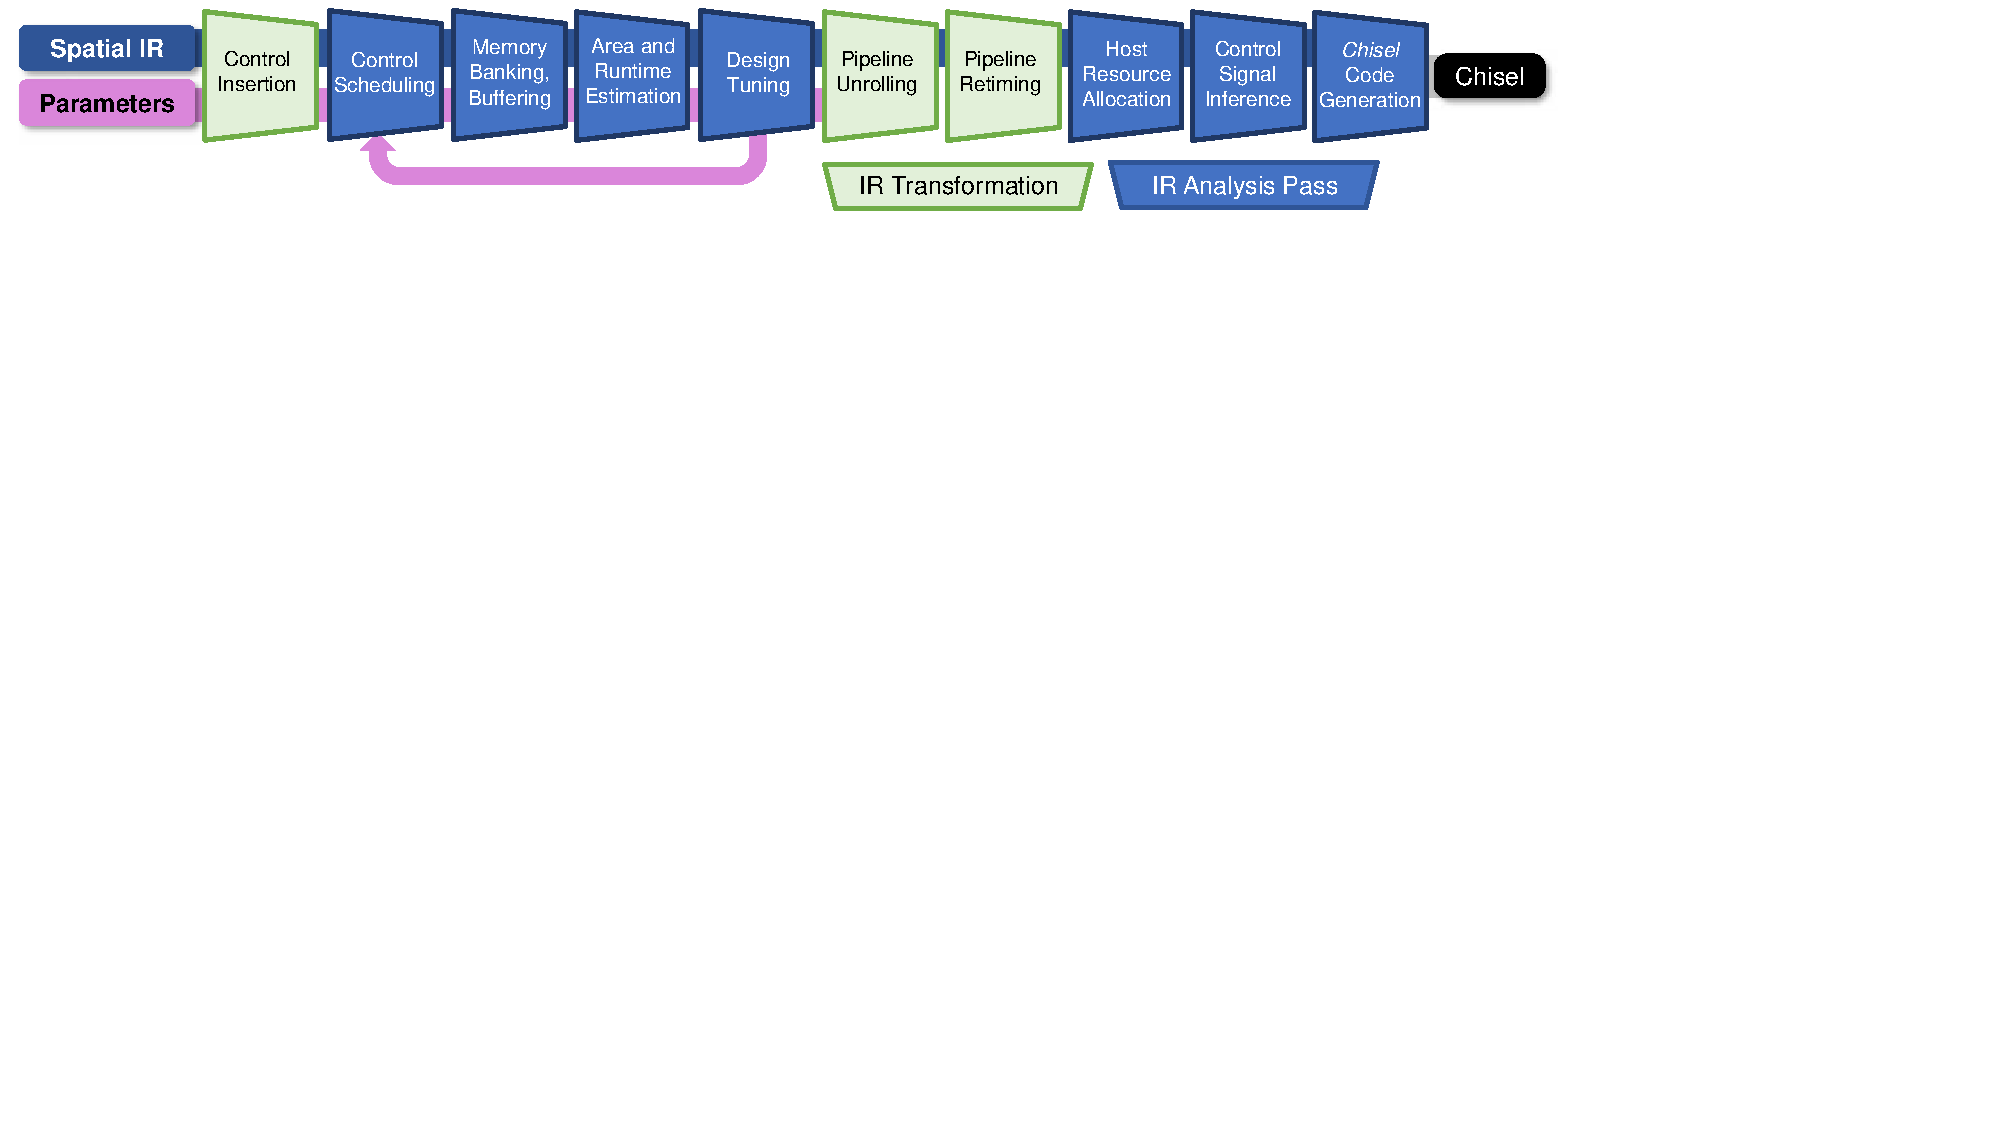
\includegraphics[clip, trim=0.3cm 15.4cm 7.7cm 0.0cm, width=\linewidth]{figs/compiler_flow.pdf}
\caption{A summary of the passes in the Spatial compiler for targeting FPGAs.}
\label{fig:compilerflow}
\end{figure*}


Figure~\ref{fig:sortMerge} shows a simple implementation of a fixed size merge sort in Spatial. Here, data is loaded into on-chip scratchpad, sorted, and then stored back into main memory.
The language's distinction between on-chip and off-chip memory types makes writing and reasoning about tiled designs like this one much more natural.
This implementation uses a statically sized \texttt{\small{SRAM}} and two \texttt{\small{FIFOs}} to split and order progressively larger size chunks of the local data.
The chunk size is determined by the outermost loop on line 8, and increments in powers of two. This behavior is best expressed in Spatial as an FSM.
